%% Requires compilation with XeLaTeX or LuaLaTeX
\documentclass[aspectratio=169,10pt,xcolor={table,dvipsnames},t]{beamer}
\usetheme{UCBerkeley}
\hypersetup{colorlinks=true, linkcolor=blue, citecolor=blue, urlcolor=blue}
\usepackage{xcolor}

\title[lecture 11]{Next Generation Data Centers and Energy Management Systems}
\subtitle{Lecture 11B: Control Systems and Optimization}
\author{Prof. Thomas M. Schutzius}
\institute{Department of Mechanical Engineering}
\date{Fall 2026}

\begin{document}

\begin{frame}
  \titlepage
\end{frame}

% Uncomment these lines for an automatically generated outline.
%\begin{frame}{Outline}
%  \tableofcontents
%\end{frame}

{
\smallframetitle % small frame title
\setbeamertemplate{background}{} % Hides background for this frame
\setbeamertemplate{footline}{}   % Reclaims the bottom space

% Learning plan. Highlight in bold the item we are covering in this lecture.
\begin{frame}
	\frametitle{Learning Plan}
	\begin{itemize}
		\item Introduction to Data Center Systems and Thermodynamics 
		\item Psychrometrics and Heat Transfer
		\item Performance Metrics and Standards
		\item Applied Computational Fluid Dynamics (CFD)
		\item Liquid Cooling \& Advanced Heat Transfer
		\item Chip Cooling: Heat Conduction and Thermal Interface Materials
		\item Power Delivery and Infrastructure (Energy sources: Geothermal, Solar, Nuclear, etc.)
		\item Overview of Simulation Field; the Concept of a Digital Twin
		\item Machine Learning and Optimization Tools
		\item Modeling and Simulation of an Energy Management System
		\item \textbf{Control Systems and Optimization}
		\item Spacecraft Thermal Control
		\item Final Project Work, Peer Feedback, and Mentor Check-in 
		\item Symposium 
	\end{itemize}		
\end{frame}

% Learning objectives go here.
\begin{frame}
	\frametitle{Learning Objectives} 
		\begin{itemize}
    			\item Differentiate between Industrial Automation (PLC) and Building Automation Systems (BAS) in terms of scan rates, protocols (BACnet vs. EtherCAT), and thermal inertia.
			\item Analyze a closed-loop control system within a data center context, identifying the roles of IT load (disturbance), PID logic (controller), and cooling infrastructure (actuator).
%			\item ...%Create a reduced order model for a 2D transient heat conduction problem with heat generation
%			\item Modeling 2D transient heat conduction in heterogeneous materials.
		\end{itemize}		
\end{frame}


% Include the typical layout of a data center facility in each lecture.
\begin{frame}
	\frametitle{Typical layout of a data center facility}
		\begin{figure}
			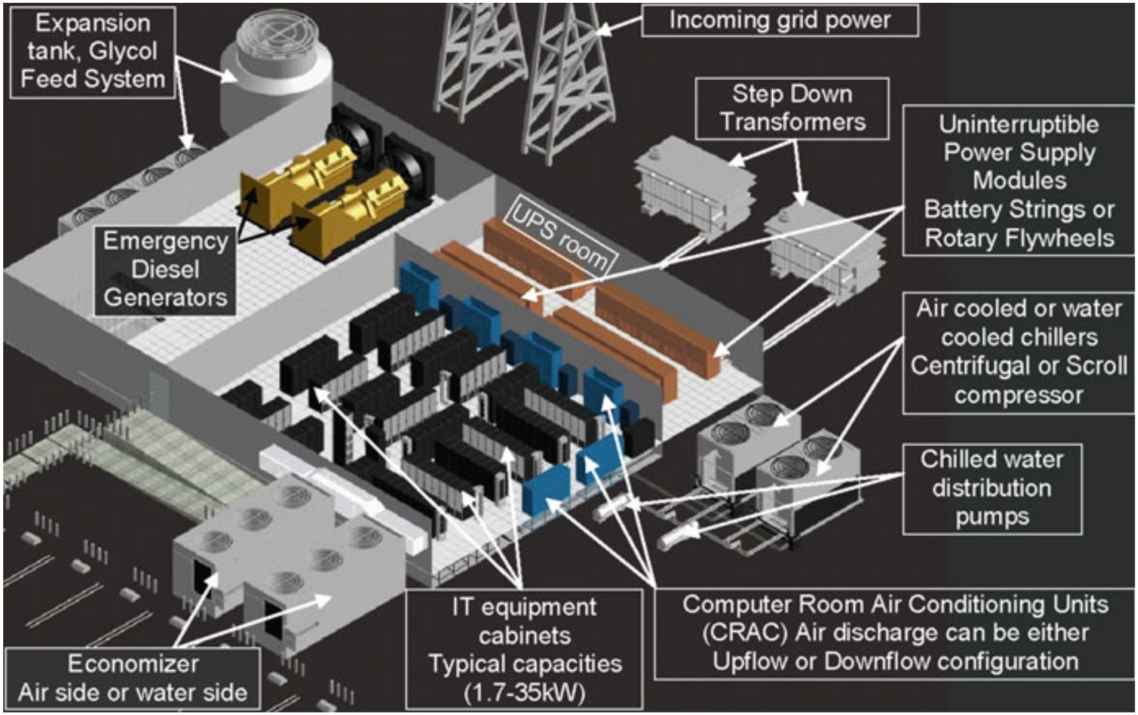
\includegraphics[width=0.65\textwidth]{../figures/joshi2021introduction-figure-01-01.pdf}
%			\vspace{-0.5cm }
		 \caption{(Figure 1.1 in Ref. \cite{joshi2012energy}).}
		\end{figure}
\end{frame}


\begin{frame}
	\frametitle{Seminar 10}
		\begin{itemize}
			\item Rama Afullo and Nelson Psenjen
			\item Title: Building Virtual AI Data Centers in Space
			\item Date: December 1, 2026
			\item Time: 15:30 (Berkeley Time)
			\item Location: GSPP 150
		\end{itemize}
\end{frame}  

    \begin{frame}
        \frametitle{Limitation of thermostats}
In a residential setting, a thermostat is a simple "bang-bang" controller (On/Off). In a Data Center, this is not a solution:

\begin{itemize}
	\item Data centers have massive thermal inertia.
	\item  If you wait for a wall-mounted thermostat to get warm before turning on a CRAC unit, the server inlets at the top of the rack have already exceeded safe operating temperatures.
	\item A data center's heat load changes instantly based on CPU/GPU utilization. We need anticipatory control, not just reactive switching.
\end{itemize}
    \end{frame}


    \begin{frame}
        \frametitle{Building Automation Systems (BAS)}
These systems orchestrate complex sequences between chillers, CRAC units, and power meters to optimize PUE. It consists of:

\begin{itemize}
	\item Server/User Interface (WebCTRL, e.g., browser-based dashboard to monitor trends, alarms, etc.)
	\item Multi-protocol routers, e.g., BACnet, {\em Modbus}
	\item Native BACnet controllers, e.g., direct digital control physically wired to sensors, e.g., temperature, humidity, pressure)
\end{itemize}
    \end{frame}

    \begin{frame}
        \frametitle{Communication protocols}
\begin{itemize}
	\item \href{https://datahub.berkeley.edu/user-redirect/git-pull?repo=https://github.com/mtsn-lab/me137-237a&subPath=examples/bacNetDataCenterCoolingDigitalTwinControlArchitectureipynb}{BACnet} is a communication protocol for building automation control (BAC). Can communicate with generators, cooling units, power distribution units, etc.
	\item Modbus is an industrial computer networking protocol, which was originally designed for programmable logic controllers (PLCs).
\end{itemize}
    \end{frame}

    \begin{frame}
        \frametitle{\href{https://datahub.berkeley.edu/user-redirect/git-pull?repo=https://github.com/mtsn-lab/me137-237a&subPath=examples/plcDataCenterCoolingDigitalTwinControlArchitecture.ipynb}{Data Center Cooling Digital Twin Control Architecture}}
%		\begin{figure}
%			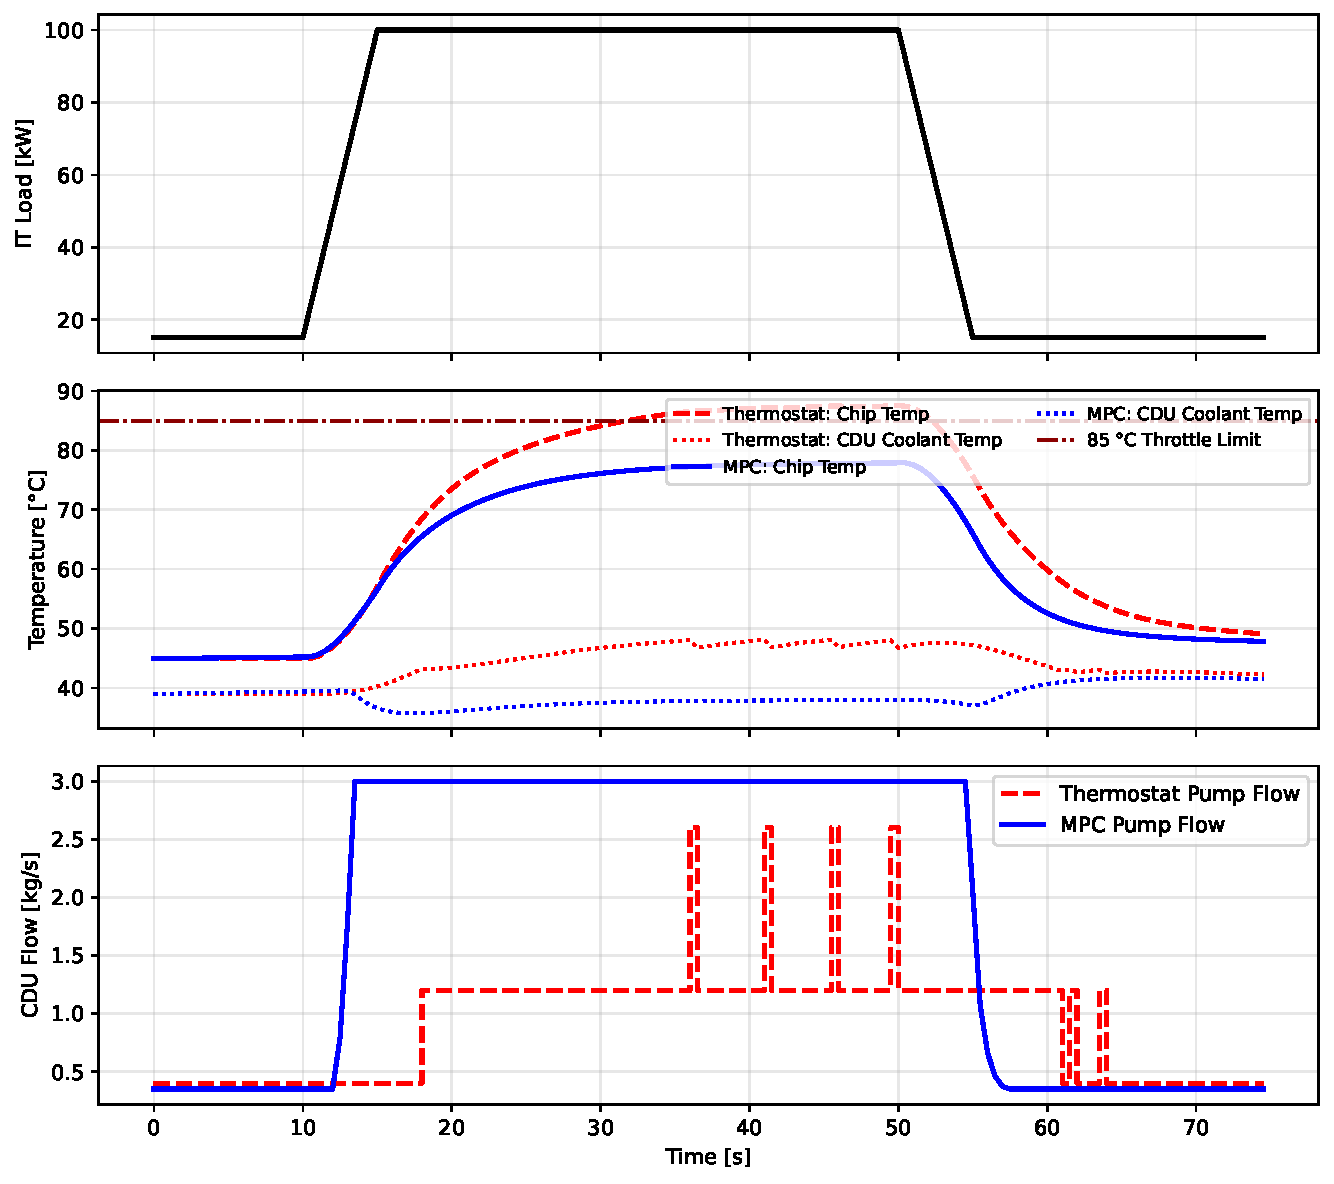
\includegraphics[width=0.45\textwidth]{../figures/modelPredictiveControlCDU.pdf}
%			\vspace{-0.5cm }
%		 \caption{CDU thermal management during an idle to full-throttle process.}
%		\end{figure}
    \end{frame}

    
%        \begin{frame}
 %       \frametitle{Conclusion}
%Moving from reactive PIDs to Predictive Control (AI-driven setpoints).

%    \end{frame}

% ------------------------------------------------------------------------------------------------------------------------------------------------------------------------------------
% This is an example for how I link the Jupyter notebook example to the slide I am showing.
% If there is a figure output from the Jupyter notebook, that should be shown here. The Jupyter notebook should be located in me137-237a/examples
% The figure output from the Jupyter notebook should go in the directory me137-237a/lectures/figures

%\begin{frame}
%	\frametitle{\href{https://datahub.berkeley.edu/user-redirect/git-pull?repo=https://github.com/mtsn-lab/me137-237a&subPath=examples/fanLaws.ipynb}{Fan Laws}}
%		\begin{figure}
%			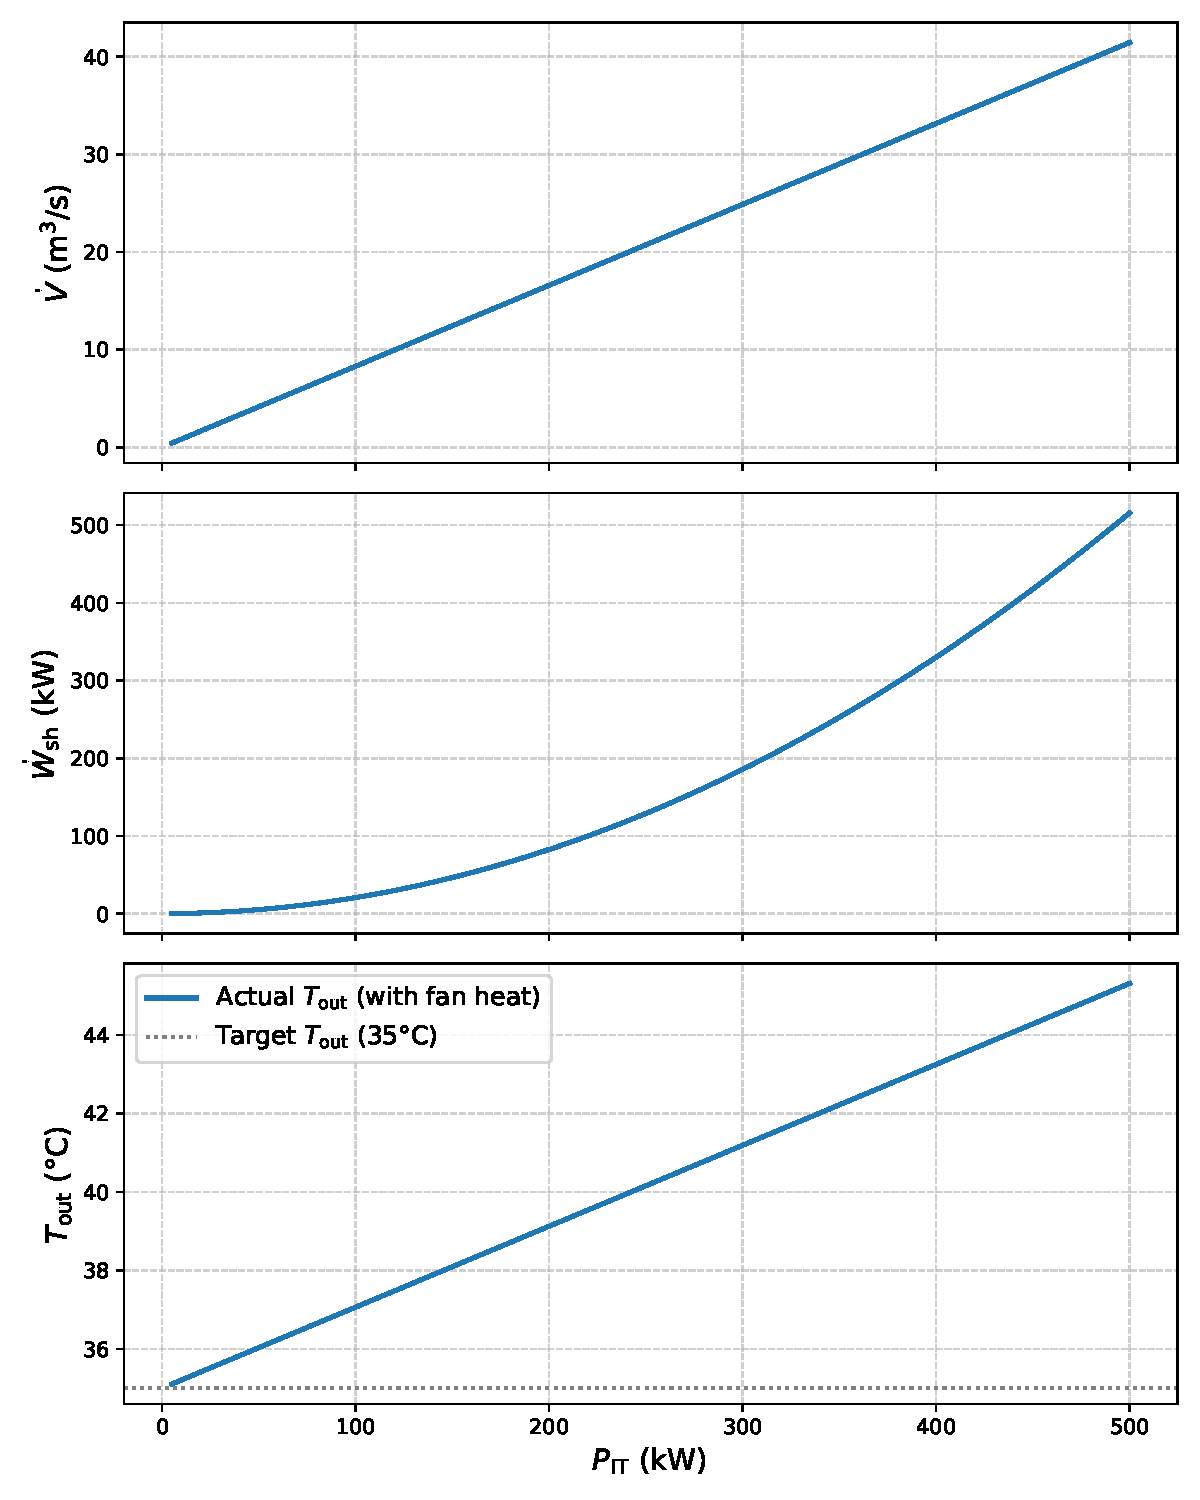
\includegraphics[width=0.4\textwidth]{../figures/rack_cooling_plots.pdf}
%		 \caption{Solution to the Pohlhausen equation. Read his biography \href{https://doi.org/10.1146/annurev.fl.16.010184.000245}{here}.}
%		\end{figure}
%\end{frame}
% ------------------------------------------------------------------------------------------------------------------------------------------------------------------------------------


{
\setbeamertemplate{bibliography item}[text] % Replaces default icons with numbers
	\begin{frame}[allowframebreaks]{References}
		\bibliographystyle{plain}
		\bibliography{../../bibliography}
	\end{frame}
}

}

\end{document}
